\documentclass[12pt]{article}
\renewcommand{\contentsname}{Inhalt}
\usepackage{graphicx}
\usepackage[margin=25mm]{geometry}
\usepackage{multicol}
\usepackage[
backend=biber,
style=numeric,
sorting=nyt,
defernumbers=false
]{biblatex}
\usepackage{hyperref}
\hypersetup{
    colorlinks=true,
    linkcolor= black,
    filecolor=black,      
    urlcolor=black,
    pdftitle={NN Portfolio Optimierung},
    pdfpagemode=FullScreen,
    citecolor=black,
    linktoc=all,
    pdfnewwindow=true,
    pageanchor=true,
    }

\graphicspath{ {./imgs/} }

\addbibresource{Literaturverzeichnis.bib}

\title{NN Portfolio Optimierung}
\date{09. Februar 2024}
\author{Patrick Spohr}
\linespread{1.5} 

\begin{document}

    \begin{titlepage}
        
        \centering
        \Huge \textbf{Neuronales Netz Portfolio Optimierung}

        \vspace{7mm}
        
        \centering
        \Large \textit{Durch die Sharpe-Quotient} 

        \vspace{7mm}

        \centering
        \large by

        \vspace{7mm}

        \large Patrick Spohr
        \vspace{2mm}
        \\ 09. Februar 2024

        \vspace{30mm}

        \centering
        \large Masterstudiengang
        \vspace{1mm}
        \\ \normalsize \textit{Finanzmathematik, Aktuarwissenschaften und Risikomanagement} 

        \vspace{5mm}

        \centering
        \large Fachbereich
        \vspace{1mm}
        \\ \normalsize \textit{Informatik, Kommunikation und Wirtschaft} 

        \vspace{5mm}

        \centering
        \large Lehrveranstaltung 
        \vspace{1mm}       
        \\ \normalsize \textit{Statistical Learning in Finance and Insurance} 

        \vspace{5mm}

        \centering
        \large Professorin
        \vspace{1mm}
        \\ \normalsize \textit{Dr. Christina Erlwein-Sayer} 


    \end{titlepage}

    \hypertarget{inhalt}{\tableofcontents}

    \newpage

    \newpage \section{Motivation} 
    
        \subsection{Portfolio Optimierung}
            
            Stellen Sie sich eine Situation vor, wobei man vielversprechende Wertpapiere fand, 
            aber er weiß nicht, wie sie in Portfolio zugeteilt werden dürfen. 
            Markowitz \cite{markowitz1952} zufolge habe das Verfahren, um Portfolio aufzubauen, zwei Schritte. 
            Am Anfang würden die einzelnen Wertpapiere geprüft, indem man Erfahrungen und Beobachtungen erwäge. 
            Danach würde man mit dieser Information ein Portfolio aufbauen. 
            Die einfachste Lösung ist die Wertpapiere mit einem Gleichgewicht versehen und 
            alles unter Fach und Dach zu bringen und warum nicht, die Wertpapiere sind gut, 
            aber das ändert das Portfolio um ein Vielfaches.
            Die Volatilität jeder neuen Wertpapiere trägt zu dem Portfolio bei und
            anschließend würde das Risiko des Portfolios erhöhen oder verringern und das könnte die Wünsche der Anleger widersprechen. 
            In Modern Portfolio Theory (MPT) sollte die steigende Volatilität eine entsprechende Rendite erwirtschaften. 

            Nun komme ich zu dem Hauptteil meiner Untersuchung. 
            Mit dem zweiten Schritt von Markowitz fange ich an, nämlich, geprüfte Wertpapiere in einem Portfolio zuzuteilen. 
            Zuerst schränke ich die Auswahl der Wertpapiere um US-Aktien ein und
            dann sollten sie zugeteilt werden, indem ein künstliches neuronales Netz und
            ein Long Short-Term Memory Layer mit der Sharpe-Quotient als Verlustfunktion eingesetzt wird. 
            Lassen Sie mich diese Begriffe und das Modell, mit dem ich die Gewichte der Aktien gerechnet habe, 
            in der Überschrift ''Methoden'' erklären.

            Im Fazit, um die Leistungen die Portfolios zu verstehen, 
            werden die optimierten Portfolios mit einem gleichgewichten Portfolio und 
            einem Vergleichsindex verglichen, weil die Leistung eines Portfolios ohne einen Maßstab keine konkrete Folgerung ergibt.

    \newpage \section{Literatur}

        \subsection{Definitionen}

            Als Einleitung definiere ich die Hauptbegriffe und deren Kurzwörter. 
            Künstliches Neuronales Netz oder KNN sind nicht-lineare Algorithmen, 
            die den Neuronen im Gehirn nachempfunden sind. 
            Die Gestalt aller KNN hat eine Eingangsschicht, 
            oft mehrere verborgenen Schichten und ein Ausgangsschicht \cite{bishop1995}. 
            Die verborgene Schicht in meinem KNN heißt Long Short-Term Memory oder
            LSTM. Man bezeichnet LSTM als eine Technik zur Verbesserung eines rekurrenten neuronalen Netzes,
            indem es um eine Art Erinnerung an frühere Erfahrungen verfügt, 
            um das Problem des verschwindenden Gradienten zu lindern \cite{hochreiter1997}. 
            Die Verlustfunktion im KNN misst den Fehler zwischen eine Beobachtung und eine Schätzung einer Regression oder einer Klassifikation. 
            Die Sharpe-Quotient, die ich als Verlustfunktion benutzte, 
            ist eine Kennzahl, die die Rendite zur Volatilität eines Portfolios zeigt \cite{sharpe1994}. 
            Zu guter Letzt ist der Risikofreier Zinssatz (Risk-Free Rate) oder RFZ,
            der in der Sharpe-Quotient eingesetzt wird, ein Referenzzinssatz, 
            der theoretisch kein Ausfallrisiko enthält. Es gibt einige RFZ, die zur Verfügung stehen,
            und ich erläutere, den ich benutzte und warum.
        
        \subsection{Literaturüberblick}
        
            Ich bespreche kurz die Literatur, die mein Projekt leiteten. 
            Die Hauptliteratur, von der ich die Idee und das Modell weiterentwickelte, 
            heißt ''Deep Learning for Portfolio Optimization'' \cite{zhang2020}. 
            Ich erkläre diese Studie ausführlicher im nächsten Teil, denn es gibt Unterschiede, 
            die ich mit meinem Projekt gegenüberstellen will. TensorFlow \cite{tensorflow2016} und 
            dessen Keras API \cite{chollet2015-keras} ermöglichte das künstliche neuronale Netz und 
            gab mir die Gelegenheit alles schnell zu erschaffen. 
            Andere Literatur war hilfreich alles zu verstehen, besonders mit den Begriffen künstliches neuronales Netz \cite{bishop1995}
            und Long Short-Term Memory von Hochreiter und Schmidhuber, die das Verfahren initiierten.

        \subsection{Hauptliteratur}
        
            Im Anschluss daran werde ich auf die wichtigen Unterschiede zwischen meinem Projekt 
            und der Studie von Zhang et al. \cite{zhang2020} hinweisen. 
            Der größte Unterschied war die Auswahl von Wertpapieren, 
            weil sie Indexfonds oder Exchange-Traded Funds (ETFs) statt Aktien auswählten. 
            Ein Portfolio mit ETFs von Aktien und Anleihen zeigt meines Erachtens die Kraft von diesem KNN-Modell nicht, 
            weil ETFs schon relativ diversifiziert und nicht volatil sind. 
            Ich wollte sehen, wie ein langfristiges Portfolio von einzelnen Aktien, 
            rücksichtslos ihre erwarteten Renditen, optimiert wird. Indexfonds erwirtschaftet in der Regel positive Rendite, 
            denn sie den Markt folgen und wirkt als eine sehr konservative Probe in diesem Experiment.

            Als Nächstes stehe ich die Sharpe-Quotient im Fokus, die sie als Verlustfunktion anwendeten. 
            Sie hatten keinen risikofreien Zinssatz in ihrem Modell benutzt, während ich ein Modell mit und ohne einen aufbaute. 
            Der RFZ ist ein wichtiger Teil die Sharpe-Quotient und kann verschiedene Ergebnisse bewirken, 
            wie in der Überschrift ''Ergebnisse'' dargestellt wird. In Hinsicht auf die Ergebnisse gibt es einen anderen Unterschied, 
            den ich erwähnen muss, weil ich keine Handelskosten betrachte. Das lässt sich als eine wichtige Auslassung zeigen, 
            denn die Aktien im ganzen Portfolio werden regelmäßig komplett wieder zugeteilt. 
            Wegen dieser Berücksichtigung wurde zumindest ein Monat lang gewartet, 
            bis die Gewichte des Portfolios wieder optimieret wurden.

    \newpage \section{Ziele}
    
        \subsection{Hauptziele}
        
            Im Folgenden gehe ich auf die Hauptziele meines Projektes. 
            Was hatte ich am Ende vor, zu erzielen? 
            Am wichtigsten werden Portfolios von beliebigen Aktien durch die Sharpe-Quotient mit und
            ohne einen RFZ optimiert. Das heißt genau, dass ich die Gewichte jeder Aktie für einen Zeitraum erzeuge. 
            Dadurch, dass ich die Portfoliowerte bekomme, multipliziere ich die Gewichte und Aktienkurs. 
            Danach werden die Leistung von den optimierten Portfolios mit einem gleichgewichtigen Portfolio und 
            einem Vergleichsindex verglichen. 30 Jahre über kann ich die monatliche Rendite jedes Portfolio rechnen, 
            um die Sharpe-Quotient jedes Portfolio auszurechnen. 
            Ich hatte keine Annahme, weil mein Projekt weit weg genug von der Hauptliteratur \cite{zhang2020}, 
            dass ich nicht wusste, ob die optimierten Portfolios besser als ein gleichgewichtiges Portfolio oder 
            ein Vergleichsindex würden. Im besten Fall würden die optimierten Portfolios dem Vergleichsindex überlegen sein.

        \subsection{Grenzen und Vermutungen}
    
            Wie ich gerade erwähnt habe, wird das Portfolio nur mit Aktien aufgebaut. 
            Angesichts dieser Bedingung schränke ich den Umfang des Portfolios weiter, 
            um zu verständlichen Schlüssen zu führen. Zuerst kommen alle Aktien aus demselben Börse, NASDAQ, also nur US-Aktien. 
            Zweitens werden die Aktien beliebig ausgewählt, die im Zeitraum 1990-2019 stetig gehandelt wurden. 
            Von diesen Grenzen folgen die Vermutungen, dass alle Aktien schon geprüft wurden und zumindest zahlungsfähig waren,
            weil sie für 30 Jahre auf dem Markt gehandelt wurden. 
            Konkret bedeutet, dass die Analysten in der Lage waren, Unternehmen zu vermeiden, die bankrottgegangen waren. 
            Das ist wichtig, weil das Modell nur funktioniert, wenn die Form die Daten gleich sind oder anders gesagt, 
            die Anzahl der Tage auf dem Markt gleich sind. Außerdem wählte ich US-Treasury Staatsanleihen als einen RFZ, 
            weil ich nur US-Aktien haben.
        
    \newpage \section{Daten}
            
        \subsection{Daten und Quellen}
    
            Ich gehe nun über zu den Daten und beschriebe, woher ich die Daten bekomme und was ich aus den Daten auszog. 
            Zusammenfassend hatte ich drei Datenquellen: Kaggle, Yahoo! Finance, und FRED, der für Federal Reserve Economic Data steht. 
            Ich erhaltete den täglichen Aktienpreis und Datum aus Stock Market Dataset auf Kaggle \cite{onyshchak}.
            Der Vergleichsindex ist der S\&P 500 und kommt aus Yahoo! Finance \cite{yahoo}. 
            Es ist zum Bemerken, dass der Ticker GSPC heißt. Aus dem GSPC erhaltete ich auch den täglichen Indexpreis und Datum. 
            Zuletzt bekam ich den risikofreien Zinssatz, 10-Year US Treasury Yield, von FRED \cite{fred}. 
            Der RFZ hat ein Datum und ein tägliches Prozent. Seltsamerweise gab ein paar Lücken im Datensatz von FRED und 
            ich musste deswegen die füllen, indem ich der Durchschnitt von dem frühen und nächsten Prozent rechnete. 
            Ich denke, das beeinflusst die Ergebnisse nicht viel, weil es sich über 30 Jahren erstrecken, aber ich mitteile es trotzdem.
            
        \subsection{Überblick der zehn beliebigen Aktien}
    
            Bei den Aktien steht die Frage im Mittelpunkt, ob sie wirklich ein typisches oder realistisches Portfolio ähneln. 
            Obwohl sie beliebig ausgewählt wurden, fand ich es wichtig, 
            die relevant Information über sie auszurechen, weil es passieren könnte, dass das Portfolio, 
            egal von den Gewichten, den S\&P 500 komplett übertrifft, wenn es Ausreißer wie Monster Beverage Corp (MNST) enthält, 
            der über 150.000\% Gesamtrendite von 1990 bis 2019 einbrachte.

            
          
            \begin{table}[htp]
                \begin{center}
                    
                    \begin{tabular}{ | l | l | l | l | l | }

                        \hline
                        \textbf{Ticker}      & \textbf{Name}                             & \textbf{Geschäft} \\
                        \hline
                        COHR                 & Coherent, Inc.                            & Laser \\
                        CTB                  & Cooper Tire \& Rubber Company             & Reifen \\
                        EQT                  & EQT Corporation                           & Energie \\
                        GOLD                 & Barrick Gold Corporation                  & Bergarbeit \\
                        NSEC                 & National Security Group, Inc.             & Versicherung \\
                        OTTR                 & Otter Tail Corporation                    & Energie \\
                        PEP                  & PepsiCo, Inc.                             & Getränke \\
                        SKYW                 & SkyWest, Inc.                             & Fluglinie \\
                        SNFCA                & Security National Financial Corporation   & Lebensversicherung \\
                        WY                   & Weyerhaeuser Company                      & Abholzung \\
                        \hline

                    \end{tabular}

                \end{center}
            \end{table}

            Aus aller beliebig ausgewählten Aktien ist SkyWest, Inc. am besten, 
            der die Summe aller monatlichen Renditen 635,7\% erwirtschaftete und
            eine durchschnittliche monatliche Sharpe-Quotient 0,825 hatte.
            Alle Aktien im Portfolio hatten eine durchschnittliche monatliche Sharpe-Quotient zwischen null und eins,
            also es gibt keine außergewöhnliche Aktie. Die Aktien gehörten zu verschiedenen Industrien und
            deswegen ist das Portfolio diversifiziert in dieser Hinsicht. Die Aktien in der Tabelle oben baute das Portfolio auf,
            das ich im Modell eingesetzt hatte.

    \newpage \section{Methoden}

        \subsection{Künstliches Neuronales Netz}

            Dieser Abschnitt behandelt die wichtigen Teile eines künstlichen neuronalen Netzes, 
            besonders ein Feed-Forward KNN. Das KNN hat drei Teile: 
            eine Eingangsschicht \( x_1, ..., x_d \ \textrm{mit d Inputs} \),
            eine oder mehrere verborgenen Schichten, \( z_1, ..., z_M \ \textrm{mit M Hidden-Units} \),
            und eine Ausgangsschicht \( y_1, ..., y_c \ \textrm{mit c Output-Units} \).
            
            \begin{figure}[htp]
            
                \begin{center}

                    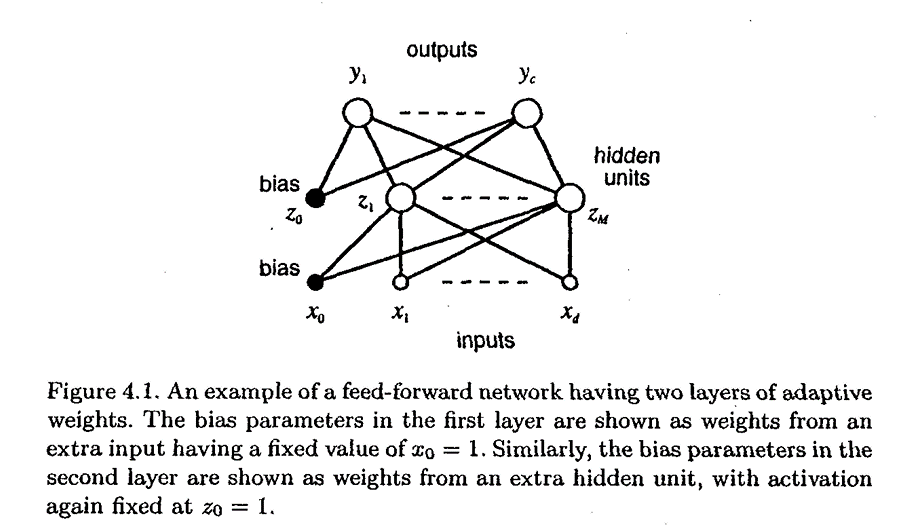
\includegraphics[scale=1]{neuronales-netz-bishop.png}
                    \caption{Feed-Forward Neuronales Netz \cite{bishop1995}}
        
                \end{center}
                
            \end{figure}
        
            Daten fließen in der Eingangsschicht, wo die Eingabe und die Gewichte jeder Neuronenverbindung multipliziert werden, 
            um eine Ausgabewert zu ergeben. 
            Für jedes Neuron wird der Aktivierungszustand durch eine Aktivierungsfunktion mit dessen Eingabewert bestimmt, 
            sodass ein Neuron feuert oder ruht. Die Ausgabe dieser Aktivierungsfunktion geht weiter in den nächsten Schichten und wie vor, 
            dieselben Verfahren gebrauchen, bis die Ausgangsschicht, wobei der Fehler der Schätzung durch eine Verlustfunktion gerechnet wird. 
            Dann fängt Back-Propagation an, wo, von hinten nach vorne, die Gewichte jeder Neuronenverbindung 
            mit Hilfe des Fehlers durch ein Gradientenverfahren aktualisiert werden. 
            Diese Feed-Forward und Back-Propagation Verfahren wiederholen sich, bis der Fehler minimisiert ist. 
            Die Training-Genauigkeit sollte in der Regel nicht viel größer als die Validation-Genauigkeit,
            weil das Over-Fitting bedeuten könnte und weist darauf, dass das Modell dem Geräusch oder der Varianz folgt.

        \subsection{Long Short-Term Memory}

            Die verborgene Schicht meines Modelles ist LSTM und ich erkläre die Wichtigkeit dieser Weiterentwicklung des KNN-Verfahrens. 
            Lassen Sie mich zuerst kurz die Schwäche vom traditionellen Feed-Forward Verfahren hervorheben. 
            Feed-Forward KNN hat sogenannt kurze Erinnerung oder ''Short-Term Memory,''
            weil die Neuronen keine Informationen über frühere Neuronen verfügen. 
            Normalerweise ist das kein Problem, weil die frühere Information keinen großen Einfluss auf die nächste Information haben. 
            Das ändert sich, wenn Zeitreihen als Eingangsdaten einfließen, 
            weil die früheren Daten wichtige Information enthalten, die die Ergebnisse verbessern können. 
            Zum Beispiel sind Aktienkurse Zeitreihen und die früheren Preise beeinflussen die nächsten. 
            
            \begin{figure}[ht]
            
                \begin{center}

                    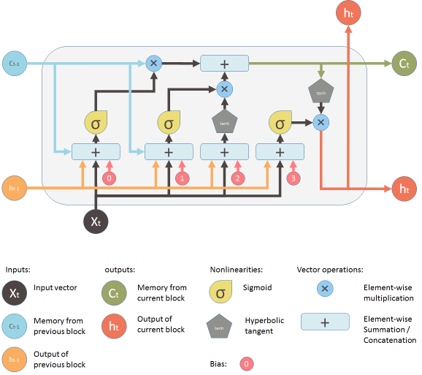
\includegraphics[scale=0.6]{lstm-yan.png}
                    \caption{Long Short-Term Memory Unit \cite{yan2016}}
        
                \end{center}
                
            \end{figure}

            Kurz gesagt, LSTM wurde gebildet, um Back-Flow-Problemen von Feed-Forward KNN ''Short-Term Memory'' zu lindern. 
            Dadurch, dass ich das beste Verfahren für meine Daten benutzen will, 
            wendete ich, wie meine Hauptliteratur \cite{zhang2020}, LSTM an. 
            Ich bemerke auch, dass LSTM eine Art rekurrentes neuronales Netz oder RNN ist, 
            weil die Ausgaben der früheren Neuronen erinnert werden. Im RNN heißt Back-Propagation unter einen anderen Namen: 
            ''Back-Propagation Through Time'' oder BPTT. 
            Der Grundidee bleibt wie vor, aber das Verfahren nutzt eine Reihe von Zeitschritten mit Eingaben und Ausgaben Paare und 
            rechnet die kumulierten Fehler über jeden Zeitschritt \cite{brownlee2020}.

        \subsection{Softmax-Funktion}

            Wie früher erwähnt hat KNN eine Aktivierungsfunktion. Mein Modell benutzte die Softmax-Funktion, 
            die eine normalisierte Exponentialfunktion ist. 
            
            \[ \sigma(x)_j = \frac{e^{z_j}}{\sum_{k=1}^{K} e^{z_k}} \ \ \textrm{für j = 1,..,K und x = Input Vektor}  \]
            
            Die Softmax-Funktion wird eingesetzt, 
            um eine Wahrscheinlichkeitsverteilung über alle unterschiedlichen möglichen Ereignisse zu rechnen. 
            Die Funktion versichert für Klassifikation mit mehr als zwei Klassen, 
            dass die Wahrscheinlichkeit aller Klassen eins ergibt und das ist wichtig für die Gewichte der Aktien im Portfolio, 
            weil die Summe aller Gewichte auch eins ist. Es ist sinnvoll zu erwähnen, 
            dass die Softmax-Funktion der Sigmoid-Funktion ähnelt aber die Summe aller Werte in der Sigmoid-Funktion nicht eins ist.

            \begin{figure}[ht]
            
                \begin{center}

                    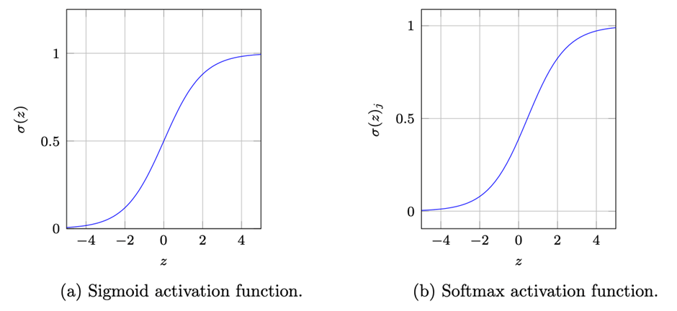
\includegraphics[scale=0.6]{sigmoid-datacamp.png}
                    \caption{Long Short-Term Memory Unit \cite{data-basecamp}}
        
                \end{center}
                
            \end{figure}

        \subsection{Sharpe-Quotient}

            Anschließend stelle ich die Sharpe-Quotient vor, die als Verlustfunktion verwendet wird. 
            Die Sharpe-Quotient enthält drei Teile: die Rendite des Portfolios, 
            ein risikofrier Zinssatz und die Volatilität oder die Standardabweichung der Renditen. 
            Was sagt die Sharpe-Quotient genau? Eine Sharpe-Quotient über eins bedeutet, 
            dass das Portfolio eine Rendite mehr als der risikofreie Zinssatz erwirtschaftet und 
            deren Ergebnis großer als die Volatilität der Rendite ist. 
            Einfacherweise wird er Anleger für das Risiko hervorragend entschädigt. 
            Eine Sharpe-Quotient gleich eins zeigt, dass Renditen und Risiken in einem ausgewogenen Verhältnis stehen. 
            Unter eins zeigt eine unterdurchschnittliche Entschädigung für das entsprechende Risiko \cite{sharpe1994}.

            \begin{multicols}{2}
                
                \begin{Large} \[ Sharpe = \frac{R_p - R_f}{\sigma_p} \] \end{Large}

                \vfill

                \begin{small}

                    \noindent $R_p$ = Portfolio Renditen \newline 
                    $R_f$ = risikofreier Zinssatz \newline 
                    $\sigma_p$ = Standardabweichung der Renditen 

                \end{small}

            \end{multicols}

            In meinem Model ist A Aktien mit x Close Preis die Features und das Y Target ist das y Gewicht für jede N Aktie. 
            Typischerweise würde die Verlustfunktion minimiert aber die Sharpe-Quotient in meinem Modell wird negiert, 
            weil das Minimum von einer negierten Funktion das Maximum ist. Das Maximum von der Sharpe-Quotient bedeutet, 
            die größte Rendite für die entsprechende Volatilität des Portfolios.


        \subsection{Struktur der zwei Modelle}

            Ich bespreche kurz die überall Struktur der zwei Modelle, die ich benutzte, 
            um das monatliche Gewicht für jede Aktie zu bestimmen. 
            Das erste Modell bleibt umgeändert von dem Modell in der Hauptliteratur \cite{zhang2020}. 
            Das bedeutet, dass das Modell ein RNN mit einer LSTM-Schicht mit 64 Einheiten ist. 
            Dieses erste Modell setzt keinen risikofreien Zinssatz in die Sharpe-Quotient-Verlustfunktion ein. 
            Das zweite Modell beachtet den risikofreien Zinssatz, um der optimalen Gewichte zu generieren. 
            Die Eingangsschicht enthält die täglichen Preise und tägliche prozentuelle Änderung jede Aktie. 
            Am Ende ergibt das Modell das monatliche Gewicht für jede Aktie, die die Sharpe-Quotient optimiert.

            \begin{figure}[ht]
            
                \begin{center}

                    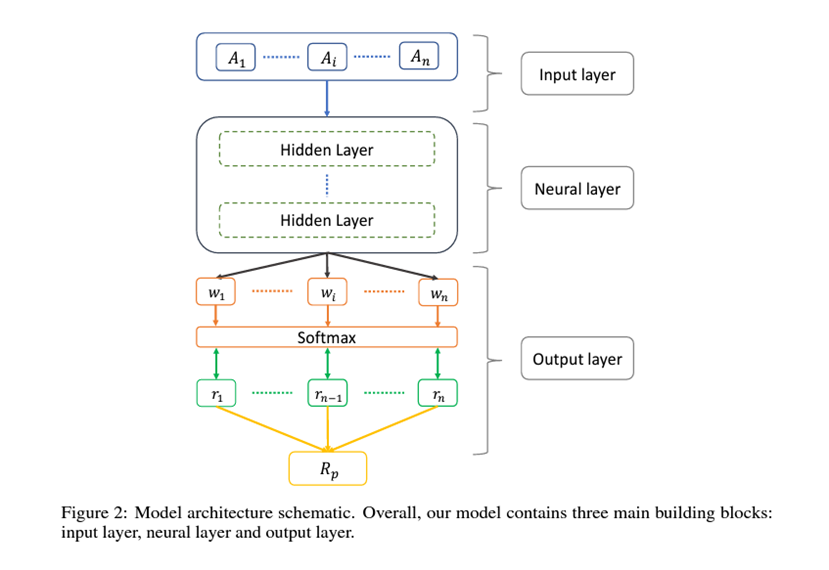
\includegraphics[scale=1]{zhang-knn.png}
                    \caption{Long Short-Term Memory Unit \cite{zhang2020}}
        
                \end{center}
                
            \end{figure}


        \subsection{Python und Keras}
                
            Um die Reproduzierbarkeit des Experiments zu dürfen, 
            liste ich alle notwendige Anwendungen und Versionen in Table \ref{pl-versionen} auf.    
            NumPy \cite{harris2020-numpy} ist wichtig für schnelle Arbeit mit Arrays und ist mit 
            pandas \cite{reback2020-pandas} \cite{mckinney2010-pandas} verbunden, um DataFrames zu erzeugen und bearbeiten. 
            Matplotlib \cite{hunter2007-matplotlib} lässt man einfach Grafik schaffen. 
            Auf TensorFlow \cite{tensorflow2016} baut sich die API Keras \cite{chollet2015-keras}, damit man Python anwenden kann.
                
                
            \begin{table}[htp]

                \begin{center} 

                \scalebox{1.2}[1.2]{
                \begin{tabular}{ | c | c | }
                \hline
                \textbf{Library}    &       \textbf{Versionen} \\
                \hline
                python              &       3.10.13 \\ 
                tensorflow          &       2.10.0 \\
                numpy               &       1.26.0 \\
                pandas              &       2.1.1 \\
                matplotlib          &       3.8.0 \\
                
                \hline
                \end{tabular}
                }

                \caption{Python und Library Versionen}
                \label{pl-versionen}

                \end{center}

            \end{table}
       

        \subsection{Monatliche Portfoliowerte}

            Um die Leistung dieses Modell zu schätzen, wurde eine Simulation durchgeführt, 
            wo man diese erzeugten Gewichte benutzen, um die Sharpe-Quotient des Portfolios zu optimieren und 
            hohe Renditen zu erwirtschaften. Die monatliche Portfoliowerte wurde gerechnet, 
            indem die optimalen Gewichte für jede Aktie im Portfolio für Zeit t, 
            wurde mit den Aktienpreisen für Zeit t+1 multipliziert. 
            Das simulierte den Aktienhandel mit Hilfe von den erzeugten Gewichten des Modelles. 
            Mit den monatlichen Portfoliowerten zur Hand konnten die monatlichen Renditen gerechnet werden. 
            Das simulierte monatliches Trading und damit konnten die monatlichen Renditen summiert, 
            um die Leistung des Portfolios auszuwerten.

            \newpage
            \begin{Large} \[ V_p = \sum_{j=1}^{A}\sum_{i=1}^{M}P^T_{i+1} \cdot w_i \] \end{Large}

            \begin{multicols}{2}
                \begin{footnotesize}
                    
                    \noindent M = 360 Monate \\
                    A = 10 Aktien \\
                    P = tägliche Preise von Aktie A im Monat M \\
                    w = monatliche Gewicht von Aktie A im Monat M \\
                    $P_{1+1}$ = Preise im Februar 1990 von Aktie A \\
                    $w_1$ = Gewicht im Januar 1990 von Aktie A 

                \end{footnotesize}
            \end{multicols}

            Insgesamt wurden vier Portfolios miteinander verglichen, 
            um die Leistungsfähigkeit des Modelles zu schätzen: S\&P 500 Vergleichsindex, 
            das gleichgewichtige Portfolio, das optimierte Portfolio ohne den risikofreien Zinssatz und 
            das optimierte Portfolio mit dem risikofreien Zinssatz. Nachdem die Renditen der Portfolios gerechnet wurden, 
            wurden die Sharpe-Quotienten jedes Portfolio gerechnet, um zu sehen, ob die Sharpe-Quotient jedes Portfolio maximiert wurde.

    \section{Ergebnisse}
    
        \subsection{Portfoliowerte und Renditen von 1990 bis 2020}

            Dieser Abschnitt beschäftigt sich mit den Portfoliowerten und Portfoliorenditen, 
            die man in diesem Experiment, besonders wenn man auf die normalisierten Portfoliowerte schaut, 
            in die Irre führen. Bei erstem Blick auf Figure \ref{n-portfoliowerte-fig} sieht man die typische Gestalt des S\&P 500s (gspc), 
            der und EQUAL eine ähnliche Linie folgen. Das Portfolio unten, OPT ohne RFZ (opt), 
            hat große Schwankungen, während OPT mit RFZ (opt\_rfr) ziemlich flach aussieht. Die optimierten Portfolios, 
            besonders OPT ohne RFZ, vielleicht keine gute Leistung gebracht -- hatte ich gedacht, 
            weil normalerweise ein steigender Portfoliowert und eine höhere Rendite verbunden sind. 


            \begin{figure}[ht]
            
                \begin{center}

                    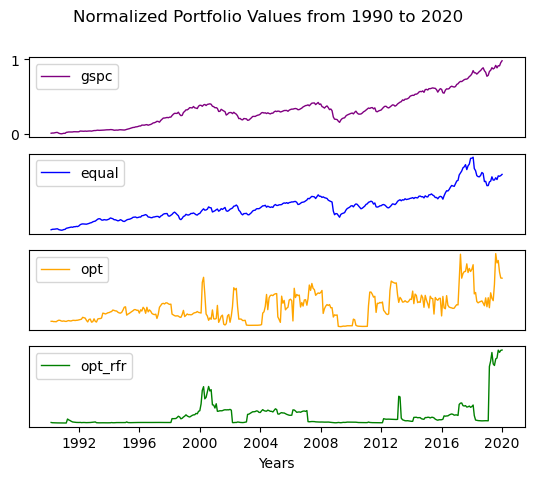
\includegraphics[scale=0.8]{normalized-portfolio-1990-2020.png}
                    \caption{Normalisierte Portfoliowerte von 1990 bis 2020}
                    \label{n-portfoliowerte-fig}
        
                \end{center}
                
            \end{figure}

            Hier musste ich nachhaken und wichtige Fragen stellen. Was hat das Modell genau gerechnet 
            und wie sollte die Ergebnisse rechnen und vergleichen? 
            Das Modell ergab die durch Sharpe-Quotient optimierten monatlichen Gewichte und 
            deswegen sollte ich die monatliche Rendite des Portfolios betrachten, weil die Vermutung steht, 
            dass man die Portfolios jeden Monat wieder zuteilen, oder einfacherweise kauft und verkauft.
            

            \begin{figure}[ht]
            
                \begin{center}

                    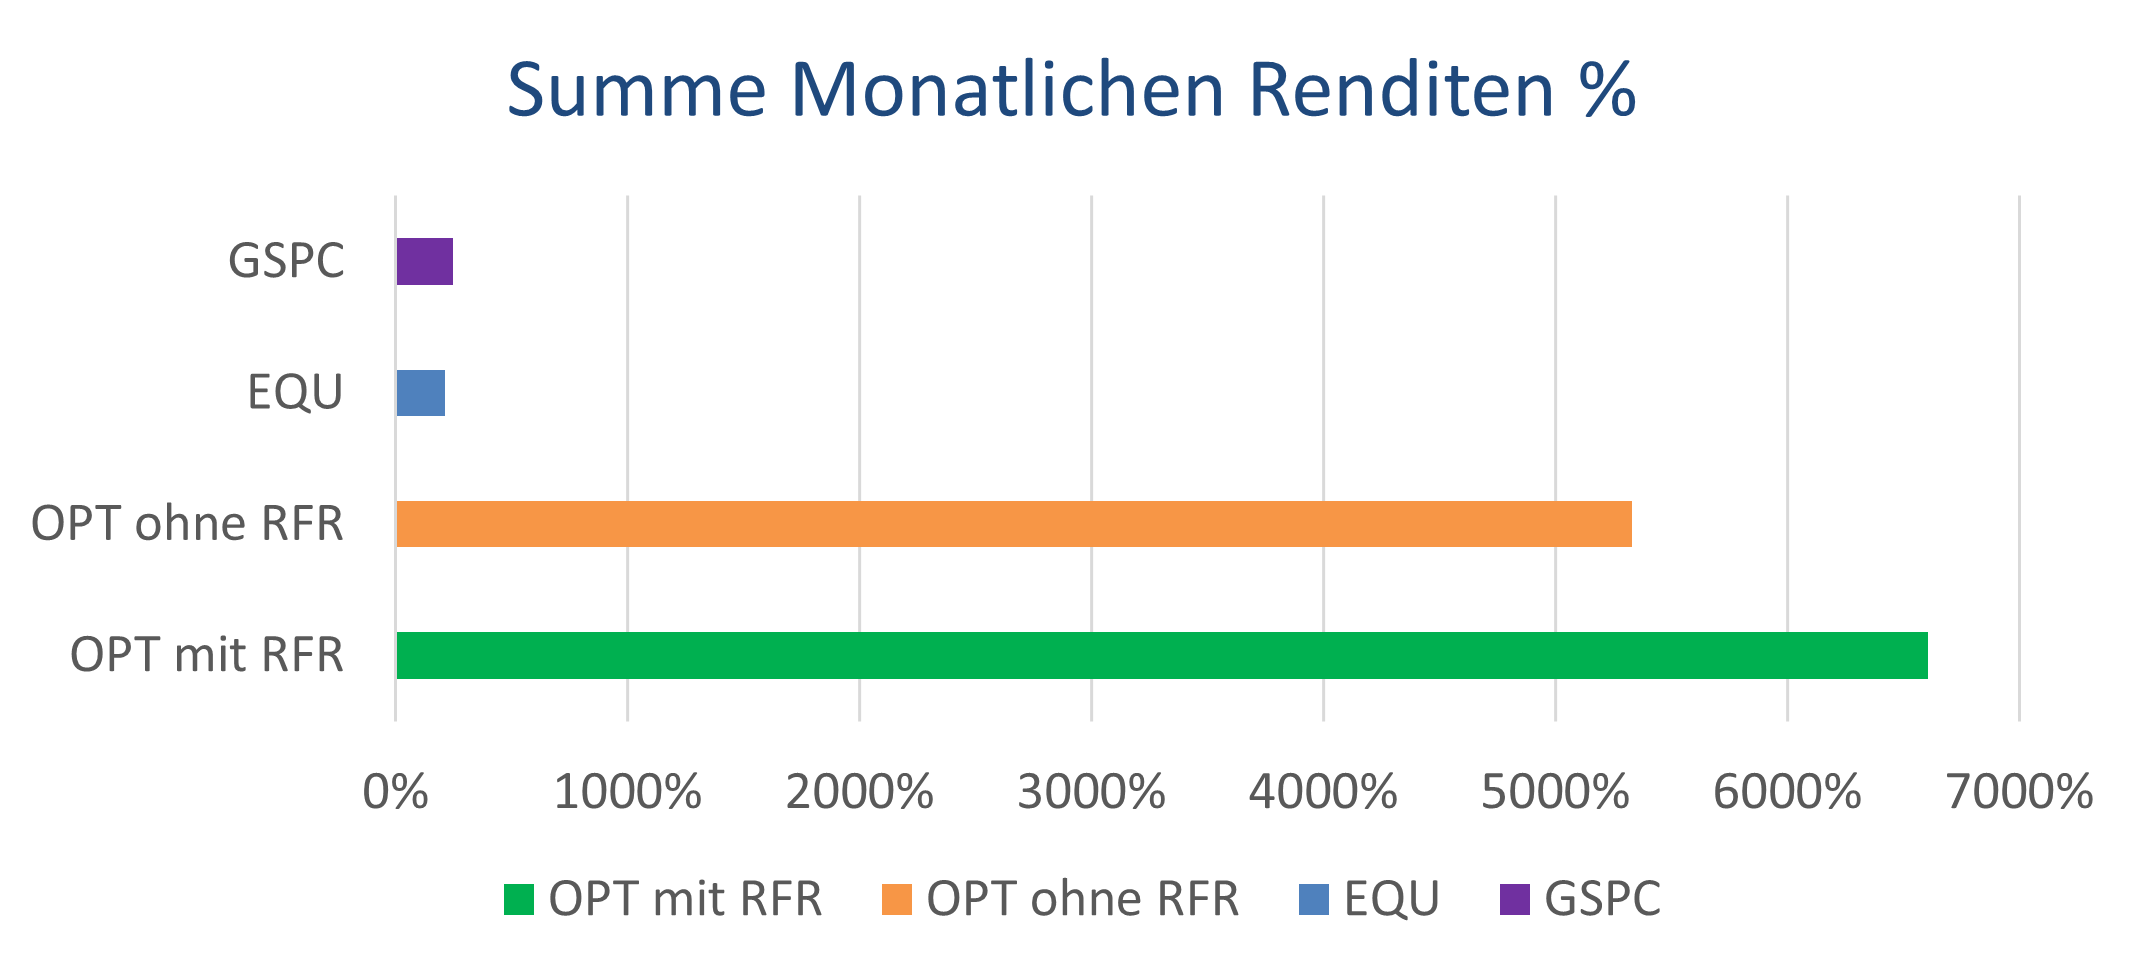
\includegraphics[scale=0.8]{summe-monatlichen-renditen-1990-2020.png}
                    \caption{Summe monatlichen Renditen von 1990 bis 2020}
                    \label{s-m-renditen-fig}
        
                \end{center}
                
            \end{figure}


            In Figure \ref{s-m-renditen-fig} und Table \ref{s-m-renditen-tab} werden sich die Unterschiede zwischen den Portfolios abgehoben. 
            Das GSPC ist EQUAL überlegen, aber hinkt den optimierten Portfolios stark hinterher. 
            Das Portfolio mit den besten Renditen ist OPT mit RFZ und ist großer als GSPC um 6.356,17 Prozent. 
            Die Einbeziehung vom RFZ hatte die Renditen in Höhe von 1.272,90 Prozent verbessert. 
            Hier muss zugegeben werden, dass die Unterschiede der Portfolios in diesem Experiment wichtiger als die Rendite selbst, 
            weil keine Handelskosten verrechnet werden und die Preise jede Aktie pro Monat gemittelt werden, 
            deshalb verliert die Ergebnisse Genauigkeit. Die GSPC und 
            GSPC haben fast gar keine Handelskosten im Verhältnis zu den optimierten Portfolios, 
            aber man kann mit einigermaßen Sicherheit sagen, dass es sich lohnt, das Portfolio zu optimieren. 

            In Hinsicht auf den Aktienkurs hatte ich später nicht nur den Mittelwert des Preises, 
            sondern auch den ersten und letzten Preis jeden Monat eingesetzt, um die monatliche Rendite zu bekommen. 
            Hier war die Ergebnisse des OPT-RFR Portfolios sogar besser, beziehungsweise 6.724,74 Prozent und 6.669,50 Prozent. 
            Diese leichte Verbesserung gilt für das GSPC-Portfolio auch, aber ich beachte diese Ergebnisse als unverbindlich, 
            weil ich die nicht genau untersucht und verglichen hatte. 
            Zusammenfassend sind die Summe prozentuale Veränderung zwischen den durchschnitten Preis jeden Monat für 
            die optimierten Portfolios viel besser als die nicht optimierten Portfolios

            \begin{table}[htp]
                \begin{center}
                    
                    \begin{tabular}{ | l | l | }

                        \hline
                        \textbf{Portfolio}   & \textbf{Summe Monatlichen Renditen \%} \\
                        \hline
                        OPT mit RFR          &      6604,73 \\            
                        OPT ohne RFR         &      5331,83 \\
                        EQU                  &      213,32 \\                 
                        GSPC                 &      248,56 \\          
                             
                        \hline

                    \end{tabular}
                    \caption{Summe Monatlichen Renditen}
                    \label{s-m-renditen-tab}
                \end{center}
            \end{table}

        \subsection{Sharpe-Quotienten}

        Als der nächste Teil meiner Untersuchung wurden die Sharpe-Quotienten für jedes Portfolio ausgerechnet. 
        Da ich zwei Modelle mit und ohne den RFZ aufgebaut hatte, 
        fand ich es in Ordnung, die Sharpe-Quotienten für jedes Portfolio 
        mit und ohne den RFZ zu rechnen (Table \ref{gs-sq-ohne-rfz} und Table \ref{md-sq-ohne-rfz}). 
        Mit diesen Parametern teilte ich die Rechnungen wieder, 
        indem ich zuerst die Summe aller Renditen durch die Standardabweichung von allen monatlichen Renditen rechnete und 
        dann alle monatliche Sharpe-Quotienten mittelte (Table \ref{gs-sq-mit-rfz} und Table \ref{md-sq-mit-rfz}). 
        Der Gewinner mit der höchsten Sharpe-Quotient ohne RFZ ist GSPC in beiden Fällen. 
        Die gesamte Sharpe-Quotient des GSPC-Portfolios ist gigantisch bei 72,302 Punkten und ist nur, 
        wenn es mit den anderen Portfolios verglichen wurden, hilfreich. 
        Interessanterweise hat OPT mit RFZ die schlechtesten Ergebnisse, -0,0026 Punkte, 
        selbst wenn die Gewichte des Portfolios durch die Sharpe-Quotient optimiert wurden.

  
                
        \begin{table}[htp]
            \begin{center}
                
                \begin{tabular}{ | l | l | }

                    \hline
                    \textbf{Portfolio}   & \textbf{Monatlicher Durchschnitt} \\
                    \hline
                    OPT mit RFR          & 39,9735  \\          
                    OPT ohne RFR         & 41,1696 \\
                    EQU                  & 52,8962  \\              
                    GSPC                 & 72,302  \\       
                            
                    \hline

                \end{tabular}
                \caption{Gesamtsumme der Sharpe-Quotienten ohne den Risikofreinen Zinssatz}
                \label{gs-sq-ohne-rfz}

            \end{center}
        \end{table}

        \begin{table}[htp]
            \begin{center}
                
                \begin{tabular}{ | l | l | }

                    \hline
                    \textbf{Portfolio}   & \textbf{Monatlicher Durchschnitt} \\
                    \hline
                    OPT mit RFR          & -0,0026 \\      
                    OPT ohne RFR         & 0,0225 \\
                    EQU                  & 0,0934 \\            
                    GSPC                 & 1,7403 \\     
                            
                    \hline

                \end{tabular}
                \caption{Monatlicher Durchschnitt der Sharpe-Quotienten ohne den Risikofreinen Zinssatz}
                \label{md-sq-ohne-rfz}

            \end{center}
        \end{table}

        Aber, als früher erwähnt, die Sharpe-Quotient ohne den RFZ ist falsch angewendet. 
        Es war mir eine Überraschung, wie viel die Ergebnisse sich umgekehrt hatten. 
        Hier hatte GSPC die schlechtesten Ergebnisse in beiden Fällen. 
        Die Sharpe-Quotient des GSPC-Portfolios ohne und mit den RFZ sank von 72,302 Punkten um 467,3736 Punkten auf -395,0716 Punkten, 
        obwohl das OPT mit RFZ Portfolio nur um 9,7243 Punkten fiel. Das OPT mit RFZ Portfolio hat die beste Sharpe-Quotient, 
        aber bei 0,08449 Punkten würde die Quotient sagen, dass die Rendite nicht genug für das Risiko wäre.

        \begin{table}[htp]
            \begin{center}
                
                \begin{tabular}{ | l | l | }

                    \hline
                    \textbf{Portfolio}   & \textbf{Monatlicher Durchschnitt} \\
                    \hline
                    OPT mit RFR          & 30,2492  \\          
                    OPT ohne RFR         & 28,7633 \\
                    EQU                  & -345,5259  \\              
                    GSPC                 & -395,0716  \\       
                            
                    \hline

                \end{tabular}
                \caption{Gesamtsumme der Sharpe-Quotienten mit dem Risikofreinen Zinssatz}
                \label{gs-sq-mit-rfz}

            \end{center}
        \end{table}

        \begin{table}[htp]
            \begin{center}
                
                \begin{tabular}{ | l | l | }

                    \hline
                    \textbf{Portfolio}   & \textbf{Monatlicher Durchschnitt} \\
                    \hline
                    OPT mit RFR          & 0,08449 \\      
                    OPT ohne RFR         & 0,08034 \\
                    EQU                  & -0,9651 \\            
                    GSPC                 & -1,1035 \\     
                            
                    \hline

                \end{tabular}
                \caption{Monatlicher Durchschnitt der Sharpe-Quotienten mit dem Risikofreinen Zinssatz}
                \label{md-sq-mit-rfz}

            \end{center}
        \end{table}

        
        \newpage \subsection{Fazit und Weiterentwicklung}

        Die Ergebnisse der Portfolios lässt mich zu dem Schluss kommen, 
        dass die Wichtigkeit von passenden Gewichten im Aktienportfolio nicht unterschätzt werden sollte. 
        Selbst beliebig ausgewählte Aktien gute Renditen erwirtschaften könnten, wenn sie im Portfolio passend zugeteilt würden. 
        Insgesamt hatte die Sharpe-Quotient als Verlustfunktion gut funktioniert, um die monatlichen Renditen anzusteigen, 
        aber die Sharpe-Quotient der optimierten Portfolios, gegen alle Erwartungen, bleibt niedrig. 
        Das RFZ im Modell ergibt viel besser monatlichen Renditen als ohne. 
        Abschließend brachte das optimierte Portfolio mit RFR über 30 Jahre jährliche Rendite von 220,16 Prozent ein.

        Dieses Projekt ergibt sich einginge Weiterentwicklungen aus. 
        Als nächster Schritt kann man ein nicht KNN-Modell benutzen, um die Unterschiede der Ergebnisse zu untersuchen. 
        Außerdem lässt dieses Verfahren sich skalieren und könnte mit mehr als 10 Aktien benutzt wird. 
        Ein Modell mit nur zehn Aktien wird oft bei einer Aktie übernommen, 
        aber bei erster Probe wird die Allokationen des Portfolios mehr verteilt, als die Anzahl der Aktien größer war. 
        Vielleicht hätte das Modell unter Over-Fitting gelitten, weil fünfzig Epochen zu viel wären, 
        deswegen kann man die Hyperparameter des Modelles verfeinern. 
        Das gilt auch für die Struktur des Modelles und hier kann man mehr LSTM-Schichten hinzufügen oder 
        die Anzahl die Einheiten in der LSTM-Schicht ändern.
    
    
    \printbibliography[heading=bibintoc, title={Literaturverzeichnis}]


\end{document}